\chapter{45. European transportation networks I}

\resp{Jules Vandendriessche}



\section{Introduction}

 Since this is a data project, the focus lays more on how the output is achieved than on its meaning.
 The data is from EuroGlobalMap and comes with a data catalogue.

 In this dataset, one finds a selection of European countries and Europe as a whole. For each of this countries files are provided for different topological attributes, of which 2 are of our main interest, node-like and edge-like.
 Examples of node-like would be stations and airports while examples of edge-like are country borders and roads. Node-like data sets exists out of a geological point with attributes, while edge-like has 2 points and attributes. According to the catalogue, every edge has to start and finish at a gives node in one of the node files. 
 
 The goal of this project is to reconstruct the rail network of the given countries and of Europe.

\section{Results and discussion}

Before constructing the network, one has to ask itself what kind of network it is interested in. In the case of a train network, one can be interested in the network decoupled from the physical topology. Meaning that all nodes are stations and an edge between nodes exists if the stations are directly connected without going through another station and disregards everything else. However, a train network has more than only stations, level crossings, merges and ports do play a role in the network. 
In this task, I opted to go for the second one.

Practically this mean a reversal of the problem, instead of connecting the stations through the edges,  the edges start and finish points are taken as nodes and stations are connected to these nodes.
These nodes can be a number of other things. From the catalogue one finds that these are: Exits, ferry stations, level crossings and airports.

Furthermore, in the data one finds that "Railroad lines can only touch at their ends and must not overlap each other." No file is found to pinpoint these points. One could make use of the exclusion principle and name the unknown points 'rail merges', but I opted to call them unknown. Note that rails are given 3D information by their property 'LLE', it indicates on which level the rail can be found. When a rail is raised, the LLE goes up by one number. This is done by cutting the edge and starting a new one at the appropriate level.
\begin{figure}[H]
\begin{center}
	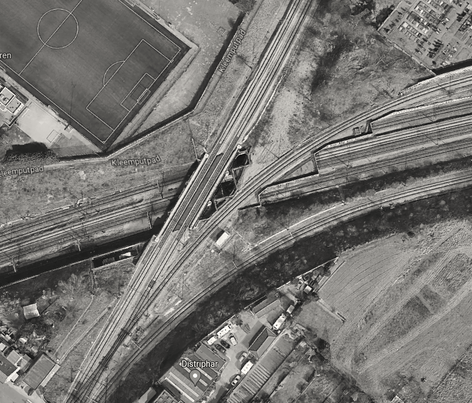
\includegraphics[width=0.6\textwidth]{rail2.png}

 
	\caption{\emph{Satellite picture of 50°53'28.0"N 4°25'19.7"E. Example of a crossing which might give trouble when reconstructing the "flow" of the network.}}
	\label{rail1.png}
\end{center}
\end{figure}
To reconstruct the network, the following algorithm has been applied:

\begin{enumerate}
    \item Use the locations and the LLE of the begin and startpoints of the provided edges to construct all possible nodes. Give these a unique ID.
    \item Check if the node locations appear in the other provided files for the nodes. If so, label the node accordingly.
    \item Edges that are raised are cut in the data. These have to be linked back together. This is done by selecting all the nodes whose location appear twice but with different LLE. Then map one ID on the other, both in the nodes file and in the edge file and delete the nodes that are mapped away.
    \item After that the data can be cleaned up. Nodes labeled "unknown" that only connect 2 edges are deleted as are double edges and self loops.
\end{enumerate}

The algorithm can be adapted such one obtains a network with only stations. 
It has been found that the dataset is not complete, as can be seen in picture \ref{rail2}.




\begin{figure}[H]
\begin{center}
	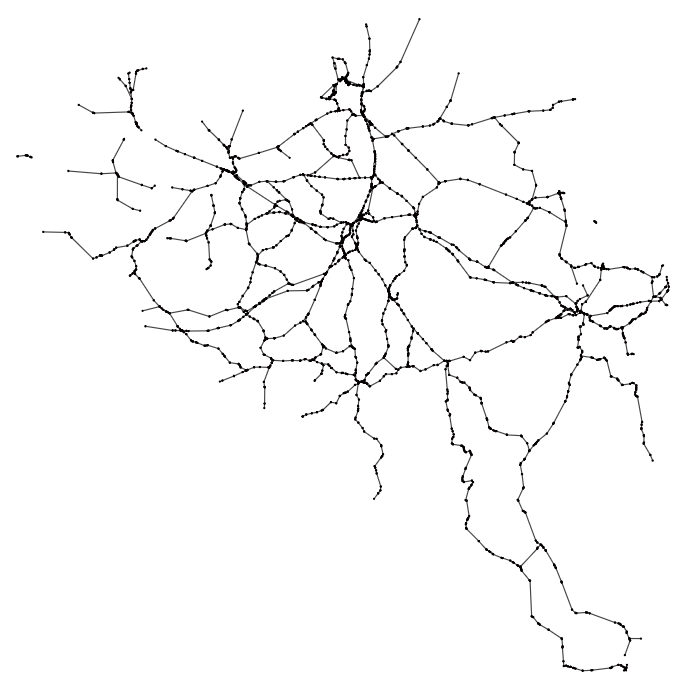
\includegraphics[width=0.6\textwidth]{rail1.png}
	\caption{\emph{ Train network of Belgium. Note the 3 disconnected components in the north-east and the lone nodes in the west. }}
	\label{rail2}
\end{center}
\end{figure}

\begin{figure}[H]
\begin{center}
	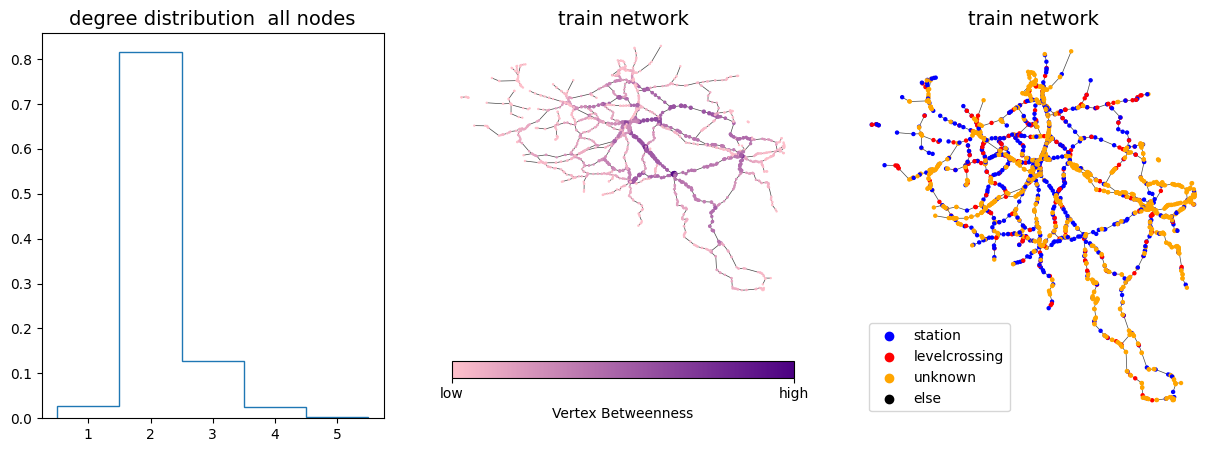
\includegraphics[width=1\textwidth]{rails4.png}
	\caption{\emph{ Train network of Belgium after applying before mentioned algorithm with node degree and betweenness. }}
	\label{rail}
\end{center}
\end{figure}
\newpage